\section{Einleitung}

Im Rahmen des Abschlussprojekts zur Vorlesung Ausgewählte Kapitel der Robotik sollen verschiedene Aufgaben rund um den Roboter UR10 der Firma Universal Robots bearbeitet werden.
Zunächst soll das Modell des Roboters in Matlab Simscape nachgebildet werden.
Dazu können die step-Dateien des Roboters verwendet werden, welche auf einigen Webseiten als kostenloser Download zur Verfügung stehen.
Die Massen und Trägheiten der Armteile bzw. Gelenke sollen dabei abgeschätzt werden.
Als Nächstes soll die zugewiesene Bewegungssequenz aus dem Beispielvideo dargestellt werden.
Die Bewegung umfasst dabei eine etwa drei Sekunden lange \en{Point to Point} Bewegung des UR10.
Eine weitere Aufgabe ist, die Drehmomentverläufe der Antriebe des Modells in Simscape auszugeben.
Als Letztes sollen die von der Simulation berechneten Drehmomente mittels einer Vergleichsrechnung mit Newton-Euler-Verfahren überprüft werden. 


Beim UR10 handelt es sich um einen 6-Achs Roboterarm, welcher in der Abbildung \ref{fig:ur10} zu sehen ist.
Sein Aufbau ist an einen menschlichen Arm angelehnt, wodurch er nahezu jede Position in seinem Arbeitsraum erreichen kann.
Er ist der größte der UR-Familie und kann Lasten von bis zu 10\,kg bei einem Arbeitsradius von bis zu 1300\,mm bewegen.
Dies ermöglicht ihm ein breites Anwendungsspektrum in der Maschinenbestückung, Palettierung und Verpackung.\cite{ur}

\begin{figure}[!htbp]
	\centering
	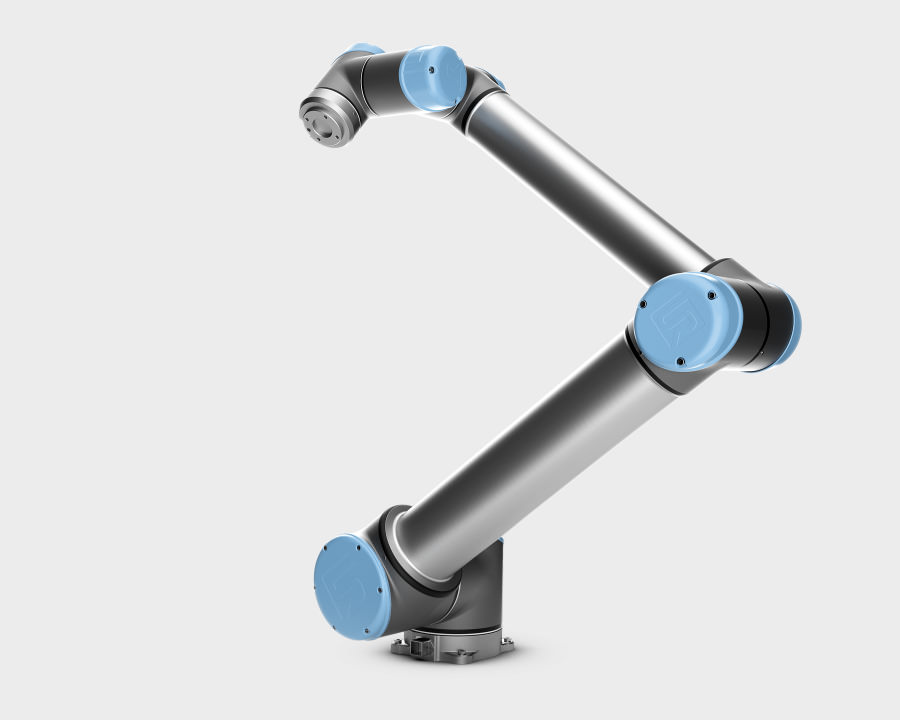
\includegraphics[width=0.7\linewidth]{grafic/ur10_universal_robots}
	\caption{UR10 der Firma Universal Robots, Quelle: \url{https://www.universal-robots.com/3d/images/slider/ur10/small_images/rendersd_00009.jpg}}
	\label{fig:ur10}
\end{figure}

